\documentclass{beamer}
\usepackage{../../Styles/Diapo}



\newcommand{\chnum}{Chapitre 11}
\newcommand{\chtitle}{Décrire un mouvement}
\newcommand{\dtype}{Cours}
\newcommand{\bgcol}{blue!2!white}


\begin{document}
% Title page frame
\begin{frame}
\titlepage
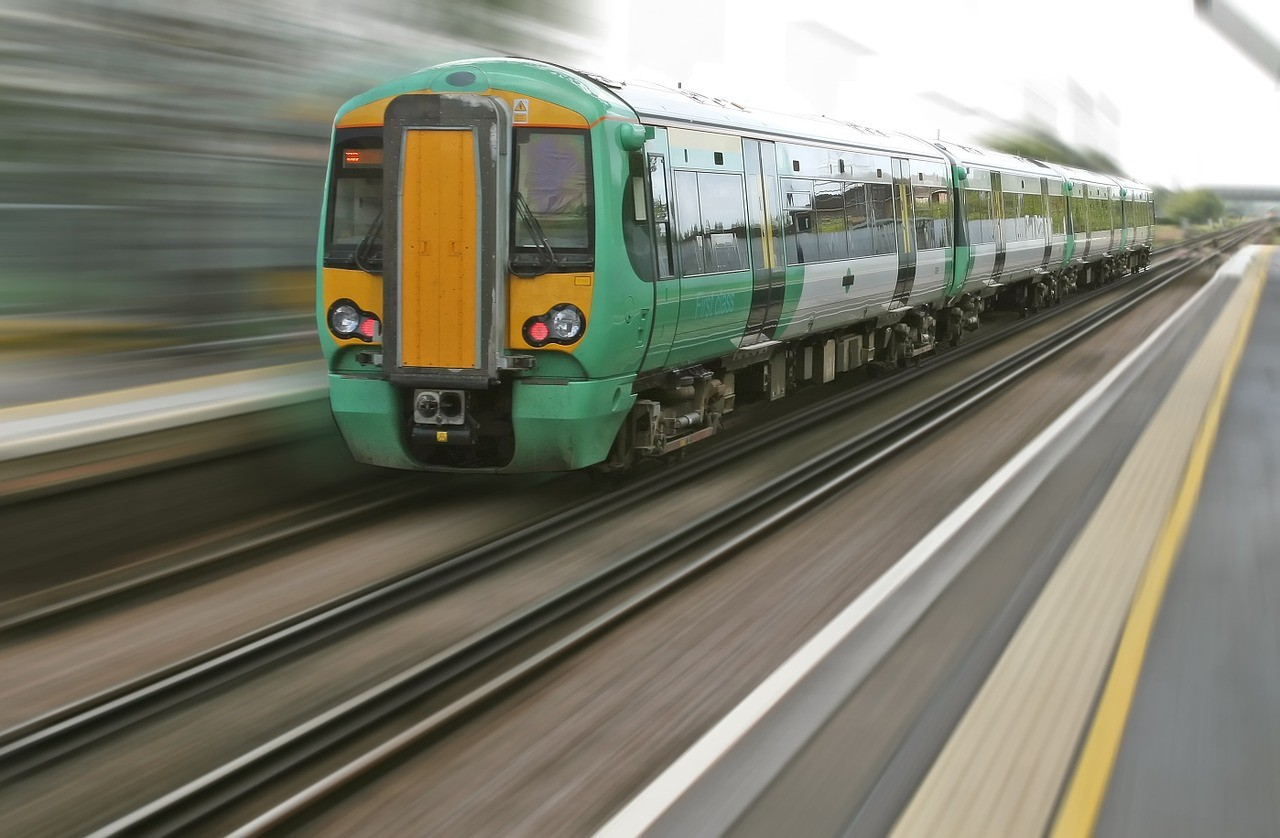
\includegraphics[width=.8\paperwidth,height=.8\paperheight]{Ressources/imagefond.jpg}
    
\end{frame}

\section{Description d'un système en physique}
%\setcounter{\section}

\begin{frame}
	\frametitle{Description d'un système en physique}
        \begin{minipage}{.4\linewidth}
		\begin{tikzpicture}
		\node[anchor=south west,inner sep=0] at (0,0) {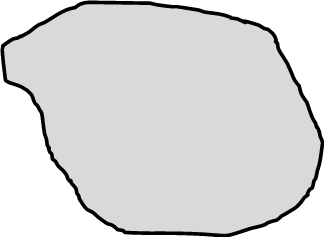
\includegraphics[width=\textwidth]{Ressources/Diapo_Fig1.png}};
		%\draw (0,0) grid(5,4);
		\node[below] (m) at (2.5,1.5) {$M$};
		\node (M) at (2.5,1.5) {+};
		\end{tikzpicture}
	\end{minipage}
        \begin{minipage}{.5\linewidth}
	Soit un objet de forme quelconque et de masse $m$.\\
	\onslide<2>
	Il sera considéré comme le \textbf{système}.\\
	%\onslide<3>
	Le centre d'équilibre de l'objet est noté $\mathbf{M}$\\
	%\onslide<4 >
	$$\downarrow$$

	Modélisation de l'objet par un point $\mathbf{M}$\\
	\end{minipage}
	
\end{frame}

\begin{frame}
	\frametitle{Inconvénients de la modélisation par un point}
	\begin{minipage}{.5\linewidth}
	Perte d'information :
		\begin{itemize}
			\item seulement des positions du barycentre
			\item manque d'informations de rotation
			\item manque les dimensions du système
		\end{itemize}
	\end{minipage}
	\begin{minipage}{.48\linewidth}
		\onslide<1->\begin{tikzpicture}[scale=.75, transform shape]
		\onslide<1-> \node[anchor=south west,inner sep=0] at (0,0) {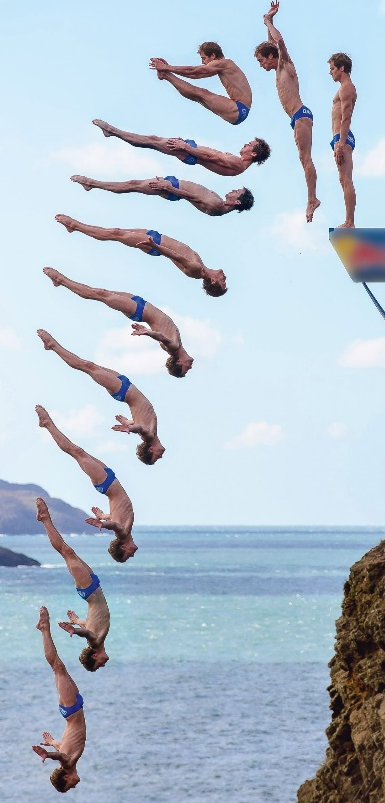
\includegraphics[width=3cm]{Ressources/Diapo_Fig2.png}};
		%\draw (0,0) grid(3,6);
		%\node[below] (m) at (2.5,1.5) {$M$};
		\onslide<2-> \node (M) at (.6,.6) {+};
		\onslide<2-> \node (M) at (.76,1.6) {+};
		\onslide<2-> \node (M) at (.9,2.45) {+};
		\onslide<2-> \node (M) at (1.1,3.1) {+};
		\onslide<2-> \node (M) at (1.2,3.8) {+};
		\onslide<2-> \node (M) at (1.3,4.4) {+};
		\onslide<2-> \node (M) at (1.44,4.85) {+};
		\onslide<2-> \node (M) at (1.5,5.1) {+};
		\onslide<2-> \node (M) at (1.9,5.6) {+};
		\onslide<2-> \node (M) at (2.3,5.45) {+};
		\onslide<2-> \node (M) at (2.7,5.3) {+};
		\onslide<1->\end{tikzpicture}
		\onslide<3->\begin{tikzpicture}[scale=.75, transform shape]
		%\draw (0,0) grid(3,6);
		%\node[below] (m) at (2.5,1.5) {$M$};
		\onslide<3-> \node (M) at (.6,.6) {+};
		\onslide<3-> \node (M) at (.76,1.6) {+};
		\onslide<3-> \node (M) at (.9,2.45) {+};
		\onslide<3-> \node (M) at (1.1,3.1) {+};
		\onslide<3-> \node (M) at (1.2,3.8) {+};
		\onslide<3-> \node (M) at (1.3,4.4) {+};
		\onslide<3-> \node (M) at (1.44,4.85) {+};
		\onslide<3-> \node (M) at (1.5,5.1) {+};
		\onslide<3-> \node (M) at (1.9,5.6) {+};
		\onslide<3-> \node (M) at (2.3,5.45) {+};
		\onslide<3-> \node (M) at (2.7,5.3) {+};
		\onslide<3-> \end{tikzpicture}
	\end{minipage}
\end{frame}

\begin{frame}
	\frametitle{Observer un lancé entre deux personnes}
	\begin{Large}
	Pour décrire le mouvement d'un système, que manque t'il ?\end{Large}
	
	\onslide<2>\begin{itemize}
		\item Selon la position de l'observateur, le mouvement sera décrit de manière différente
		\item Il faut donc fixer une "référence" pour décrire un mouvement
	\end{itemize}
\end{frame}

\section{Le référentiel}
\begin{frame}
	\frametitle{Le référentiel}
	\large
	C'est l'objet auquel on se réfère pour décrire un mouvement.\\
	En physique, il permet de définir :
    
	\begin{itemize}
		\item un système d'axes spatiaux (x,y,z) permettant de repérer la position de $M$
        \begin{minipage}{.4\linewidth}
            \begin{tikzpicture}[scale=.5, transform shape]
            \draw[-Latex](0,0) to (3,0);
            \draw[-Latex](0,0) to (0,3);
            \draw[-Latex](0,0) to (-1.5,-1.5);
            \end{tikzpicture}
        \end{minipage}
		\item une horloge permettant de mesurer le temps
        \begin{minipage}{.4\linewidth}
            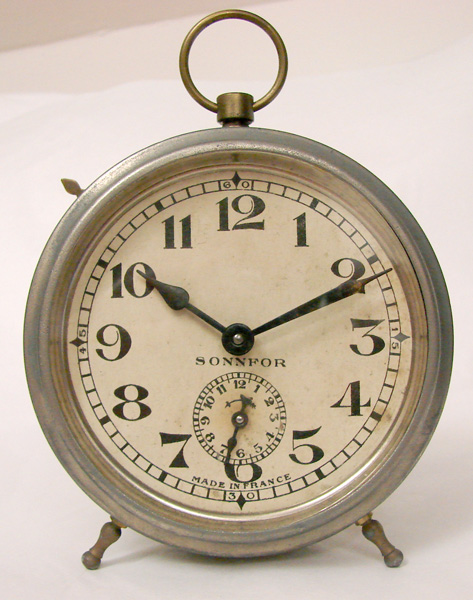
\includegraphics[width=.5\linewidth]{Ressources/reveil.jpg}
        \end{minipage}
	\end{itemize}
\end{frame}

\begin{frame}
	\frametitle{Exemples de référentiels}
	\noindent \begin{tabular}{|>{\centering}m{.24\textwidth}|m{.33\textwidth}|m{.33\textwidth}|}\hline
	\textbf{Référentiel} & \centering \textbf{Références} & \centering \arraybackslash \textbf{Utilisation}\\ \hline
	
	\textbf{Terrestre} & le sol ou un objet fixe par rapport au sol & pour étudier les mouvements à la surface de la Terre\\ \hline
	\textbf{Géocentrique} & centre de la Terre et trois étoiles très éloignées situées de manière à former des axes orthogonaux (x,y,z) & pour étudier les mouvements des systèmes proches de la Terre\\ \hline
	\textbf{Héliocentrique} & centre du Soleil et trois étoiles très éloignées situées de manière à former des axes orthogonaux (x,y,z) & pour étudier les mouvements dans le système solaire ou par rapport au Soleil\\ \hline
	\end{tabular}
\end{frame}

\section{Trajectoire et vitesse}
\begin{frame}        
	\frametitle{Trajectoire et vitesse}
	\large
	\textbf{Trajectoire :}\\	
	Tracé reliant les positions successives occupées par un point matériel durant son mouvement.\\
	
	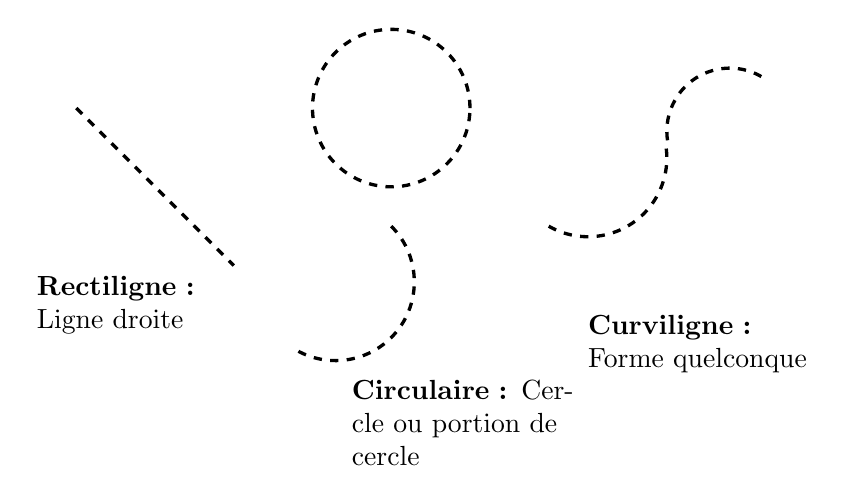
\begin{tikzpicture}
	\draw[dashed, very thick] (0,0)--(2,-2);
	\draw[dashed, very thick] (4,0) circle(1);
	\draw[dashed, very thick] (4,-1.5) arc(45:-120:1);
	\draw[dashed, very thick] (6,-1.5) arc(-120:10:1);
	\draw[dashed, very thick, rotate = 180] (-8.7,-.4) arc(-120:10:.8);
	\node[text width=3cm] (R) at (1,-2.5) {\textbf{Rectiligne :} Ligne droite};
	\node[text width=3cm] (Cir) at (5,-4) {\textbf{Circulaire :} Cercle ou portion de cercle};
	\node[text width=3cm] (Cur) at (8,-3) {\textbf{Curviligne :} Forme quelconque};
	\end{tikzpicture}
\end{frame}

\subsection{Vecteur déplacement}
\begin{frame}
	\frametitle{Vecteur déplacement}
	\begin{center}
		\begin{tikzpicture}
		\node[anchor=south west,inner sep=0] at (0,0) {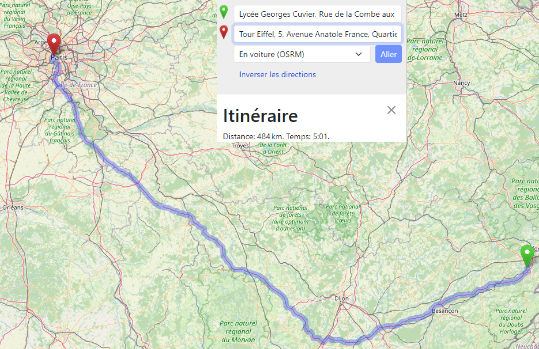
\includegraphics[width = \linewidth]{Ressources/maps2.png}};
		\end{tikzpicture}
	\end{center}
\end{frame}

\begin{frame}
	\frametitle{Vecteur déplacement}
	\begin{minipage}{.5\textwidth}
		\large C'est le \underline{vecteur de translation} reliant une position $M$ observée à un instant $t$, à une position $M'$ observée à un instant $t'$.	\\
		
		Il se note $\overrightarrow{MM'}$
	\end{minipage}
	\begin{minipage}{.48\textwidth}
		\begin{tikzpicture}
		\draw[-Stealth, thick] (0,0) to (0,5);
		\draw[-Stealth, thick] (0,0) to (5,0);
		
		\node (m1) at (.5,.5) {$\times$};
		\node (m2) at (2,3) {$\times$};
		\node (m3) at (4,4) {$\times$};
		
		\node[below right] (M1) at (.5,.5) {$M_1$};
		\node[below right] (M2) at (2,3) {$M_2$};
		\node[below right] (M3) at (4,4) {$M_3$};
		
		\draw[-Stealth, very thick, blue!60!white] (0.5,0.5) to (2,3);
		\node[below right, blue!60!white] (M1M2) at (1.25,1.75) {$\overrightarrow{M_1M_2}$};
		\end{tikzpicture}
	\end{minipage}
\end{frame}

 \subsection{Vecteur vitesse}
\begin{frame}
	\frametitle{Vecteur vitesse}
	\begin{minipage}{\linewidth}
	\centering
		\begin{tikzpicture}[scale=1,transform shape, block/.style={
draw,
fill=white,
rectangle, 
text width=15em,
align=center,
font=\small}]
		\tikzstyle{ville}=[rectangle, aspect=2.5,thick,draw=green!30!black,fill=green!30,text=black]
		
		\node[anchor=south west,inner sep=0] at (0,0) {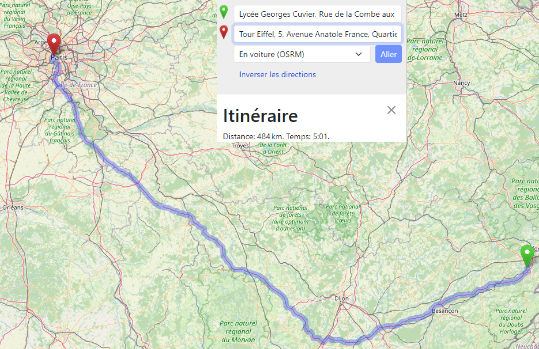
\includegraphics[width = 10cm]{Ressources/maps2.png}};
		\node[ville, above right] (Paris) at (1.5,6){$t_{Paris} = \text{13h01}$};
		\node[ville, above left] (Montbéliard) at (10,2){$t_{M^tBeliard} = \text{8h00}$};
		%\draw (0,0) grid(10,6);
		\onslide<2-> \node[block](Vit) at (3,2){\textbf{Vitesse instantanée :} \begin{itemize}
		\item Besoin de beaucoup de points très proches
		\item Complexe à déterminer 
	\end{itemize}};
		\end{tikzpicture}
	\end{minipage}
\end{frame}

\begin{frame}
	%\frametitle{Vecteur vitesse}
	\begin{minipage}{\linewidth}
	\centering
		\begin{tikzpicture}[scale=1,transform shape, block/.style={
draw,
fill=white,
rectangle, 
text width=20em,
align=center,
font=\small}]
		\tikzstyle{ville}=[rectangle, aspect=2.5,thick,draw=green!30!black,fill=green!30,text=black]
		
		\node[anchor=south west,inner sep=0] at (0,0) {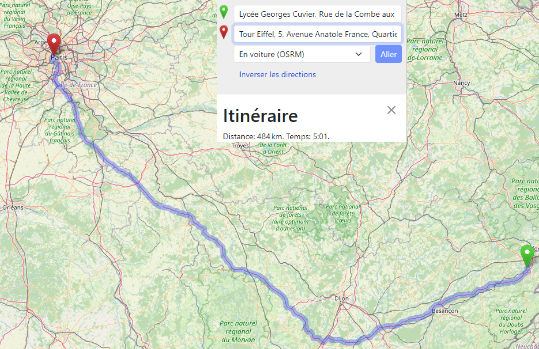
\includegraphics[width = 10cm]{Ressources/maps2.png}};
		\node[ville, above right] (Paris) at (1.5,6){$t_{Paris} = \text{13h01}$};
		\node[ville, above left] (Montbéliard) at (10,2){$t_{M^tBeliard} = \text{8h00}$};
		%\draw (0,0) grid(10,6);
		\draw[-Stealth,line width = 2pt,blue!80!black] (9.8, 1.5) to (1,5.5);
		\node[below,blue!80!black, rectangle,fill=white] (d) at (4,3.5) { $\mathbf{\overrightarrow{d_{M^tBeliard-Paris}}}$};
		\onslide<2-> \node[block](Vit) at (5,2){\textbf{Vitesse moyenne :}\\
	
	Valeur : $\dfrac{d_{M^tBeliard-Paris}}{t_{Paris} - t_{M^tBeliard}}$\\
	
	Orientation : comme le vecteur déplacement\\
	
	\textcolor{red}{Comment et où le tracer ?}};
		\end{tikzpicture}
	\end{minipage}
\end{frame}

\begin{frame}
	\frametitle{Méthode de tracé}
	\begin{minipage}{.5\textwidth}
		Il faut disposer d'au moins deux positions du système. On aura le \textbf{vecteur vitesse moyenne} d'un système au point $M_2$, à la date $t_2$ qui aura pour expression : $$\vv{v_2} = \dfrac{\vv{M_2M_3}}{t_3-t_2}$$
		Ce vecteur a les caractéristiques suivantes :
		\begin{itemize}
		\item \textbf{direction} : tangent au mouvement
		\item \textbf{sens} : celui du mouvement
		\item norme : $v_2 = \dfrac{M_2M_3}{t_3-t_2}$
		\end{itemize}
		
	\end{minipage}
	\begin{minipage}{.48\textwidth}
		\begin{tikzpicture}
		\draw[-Stealth, thick] (0,0) to (0,5);
		\draw[-Stealth, thick] (0,0) to (5,0);
		
		\node (m1) at (.5,.5) {$\times$};
		\node (m2) at (2,3) {$\times$};
		\node (m3) at (4,4) {$\times$};
		
		\node[below right] (M1) at (.5,.5) {$M_1$;$t_1$};
		\node[left] (M2) at (2,3) {$M_2$;$t_2$};
		\node[below right] (M3) at (4,4) {$M_3$;$t_3$};

            \draw[dashed] plot[domain = .5:4] (\x,-0.333*\x^2+2.5*\x-0.667);
		
		\draw[-Stealth, very thick, blue!60!white] (2,3) to (4,4);
		\node[below right, blue!60!white] (M1M3) at (2.75,2.75) {$\overrightarrow{M_1M_3}$};
		
		\draw[-Stealth, very thick, red!60!white] (2,3) to (2.75,3.8);
		\node[above, red!60!white] (M1M3) at (2.2,3.5) {$\overrightarrow{v_2}$};
		\end{tikzpicture}
	\end{minipage}
\end{frame}

\section{Décrire un mouvement}
\begin{frame}
	\frametitle{Variation de la norme du vecteur vitesse}
	\begin{minipage}{.5\textwidth}
		\begin{itemize}
			\item Si la norme du vecteur ne change pas : le mouvement est \underline{uniforme}.
		\end{itemize}
	\end{minipage}
	\begin{minipage}{.48\textwidth}
		\begin{tikzpicture}
		\draw[-Stealth, thick] (0,0) to (0,5);
		\draw[-Stealth, thick] (0,0) to (5,0);
		
		\foreach \k in {.5,1,...,4} {
		\node (m) at (\k,\k) {$\times$};
		\draw[-Stealth, thick, red!60!white] (\k,\k) to (\k+.3,\k+.3);
		}
		\end{tikzpicture}
	\end{minipage}
\end{frame}

\begin{frame}
	\frametitle{Variation de la norme du vecteur vitesse}
	\begin{minipage}{.5\textwidth}
		\begin{itemize}
			\item Si la norme du vecteur vitesse augmente, le mouvement est \underline{accéléré}.
		\end{itemize}
	\end{minipage}
	\begin{minipage}{.48\textwidth}
		\begin{tikzpicture}
		\draw[-Stealth, thick] (0,0) to (0,5);
		\draw[-Stealth, thick] (0,0) to (5,0);
		
		\foreach \k in {.5,1,2,3.5} {
		\node (m) at (\k,\k) {$\times$};
		\draw[-Stealth, thick, red!60!white] (\k,\k) to (1.5*\k,1.5*\k);
		}
		\end{tikzpicture}
	\end{minipage}
\end{frame}

\begin{frame}
	\frametitle{Variation de la norme du vecteur vitesse}
	\begin{minipage}{.5\textwidth}
		\begin{itemize}
			\item Si la norme du vecteur vitesse diminue, le mouvement est \underline{ralenti}.
		\end{itemize}
	\end{minipage}
	\begin{minipage}{.48\textwidth}
		\begin{tikzpicture}
		\draw[-Stealth, thick] (0,0) to (0,5);
		\draw[-Stealth, thick] (0,0) to (5,0);
		
		\foreach \k in {.8,1.8,3,3.5,3.75} {
		\node (m) at (\k,\k) {$\times$};
		\draw[-Stealth, thick, red!60!white] (\k,\k) to (\k+1/\k,\k+1/\k);
		}
		\end{tikzpicture}
	\end{minipage}
\end{frame}

\begin{frame}
	\frametitle{Variation de la direction et du sens}
	\begin{minipage}{.4\textwidth}
		\begin{itemize}
			\item Si la direction ou le sens du vecteur ne change pas : le mouvement est \underline{rectiligne}
			\item Si ils changent, le mouvement est \underline{circulaire} ou \underline{curviligne}.
		\end{itemize}
	\end{minipage}
	\begin{minipage}{.48\textwidth}
		\begin{tikzpicture}[scale=.7,transform shape]
		\draw (0,0) ellipse (4cm and 1.7cm);
		
		\node (F1) at (-3,0) {$\times$};
		\node[circle,fill=yellow] (F2) at (3,0) {$\times$};
		
		\node[below] (f1) at (-3,0) {Foyer 1};
		\node[below] (E) at (3,0) {Etoile};
		
		\draw[dashed, thick] (-4,0) -- (4,0);
		
		\node[circle,fill=blue] (T1) at (-4,0) { };
		\node[circle,fill=blue] (T2) at (0,-1.7) { };
		\node[circle,fill=blue] (T3) at (4,0) { };
		\node[circle,fill=blue] (T4) at (0,1.7) { };
		
		\draw[-Stealth, red, thick] (-4,0) to (-4,-2);
		\node[red, left] (v1) at (-4,-1){$\overrightarrow{v_1}$};
		
		\draw[-Stealth, red,thick] (0,-1.7) to (2,-1.7);
		\node[red, below] (v2) at (1,-1.7){$\overrightarrow{v_2}$};
		
		\draw[-Stealth, red, thick] (4,0) to (4,2);
		\node[red, right] (v3) at (4,1){$\overrightarrow{v_3}$};
		
		\draw[-Stealth, red,thick] (0,1.7) to (-2,1.7);
		\node[red, above] (v4) at (-1,1.7){\Large $\overrightarrow{v_4}$};
		\end{tikzpicture}\\
		Exemple d'une planète en orbite elliptique autour d'une étoile.
	\end{minipage}
\end{frame}

\begin{frame}
	\frametitle{Description d'un mouvement}
	\begin{small}
		\begin{tabular}{|>{\centering}m{.3\linewidth}|>{\centering}m{.18\linewidth}|>{\centering}m{.18\linewidth}|>{\centering\arraybackslash}m{.18\linewidth}|}
			\hline
			\diagbox{Dir./sens}{Norme} & Diminue & Ne varie pas & Augmente \\
			\hline
			Ne change pas & Rectiligne Décéléré & Rectiligne Uniforme & Rectiligne Accéléré\\
			\hline 
			Varie & Curviligne Décéléré & Curviligne Uniforme & Curviligne Accéléré\\
			\hline
		\end{tabular}
	\end{small}
\end{frame}
\end{document}